\documentclass[12pt]{article}

\usepackage[utf8]{inputenc}
\usepackage[T1]{fontenc}
\usepackage{mathptmx}
\usepackage[margin=1in]{geometry}
\usepackage{setspace}
\usepackage[right]{lineno}
\usepackage{graphicx}
\usepackage{booktabs}
\usepackage{longtable}
\usepackage{array}
\usepackage{caption}
\usepackage[hidelinks]{hyperref}

\captionsetup{font=small, labelfont=bf}
\setlength{\parindent}{0pt}
\setlength{\parskip}{6pt}
\setlength{\emergencystretch}{2em}

\newcolumntype{R}[1]{>{\raggedleft\arraybackslash}p{#1}}
\newcommand{\deltaauc}{$\Delta$AUC}

\title{}
\date{}

\begin{document}
\linenumbers

% ============================================================
% TITLE PAGE
% ============================================================
\begin{singlespace}
\begin{center}
{\Large\bfseries Reported biomarker--cognition associations do not translate into predictive utility: a pre-registered analysis of NHANES 2011--2014\par}
\end{center}

\bigskip

\begin{center}
Shreyan Kancharla$^{1,\ast}$, Neil Patel$^{2,\ast}$
\end{center}

\medskip

\noindent $^{\ast}$These authors contributed equally to this work and share first authorship.

\medskip

\noindent $^{1}$Davidson College, Davidson, NC, USA.

\noindent $^{2}$University of North Carolina at Chapel Hill, Chapel Hill, NC, USA.

\medskip

\noindent \textbf{Corresponding author:} Shreyan Kancharla, shkancharla@davidson.edu, ORCID: 0009-0009-8654-110X.

\noindent Neil Patel, ORCID: 0009-0000-6134-5641.

\end{singlespace}

\clearpage

% ============================================================
% ABSTRACT
% ============================================================
\doublespacing
\section*{Abstract}

\textbf{Background.} Multiple studies report associations between blood metals, nutritional biomarkers and cognitive performance among US adults aged 60 and over in the National Health and Nutrition Examination Survey (NHANES) 2011--2014. None isolates the biomarkers' predictive contribution beyond demographics, with calibration and decision-curve analysis.

\textbf{Methods.} We analysed NHANES 2011--2012 and 2013--2014, restricted to examined participants aged 60 and over. Low cognitive performance was defined as the lowest quartile of a composite z-score from CERAD immediate and delayed recall, animal fluency, and the Digit Symbol Substitution Test. Four nested specifications were pre-specified: demographics (M0); demographics plus five blood metals (M1); demographics plus fifteen nutritional and metabolic biomarkers (M2); and both blocks (M3). A pre-specified secondary baseline (M0+) added eight routinely recorded clinical covariates. Three algorithms (L2-penalized logistic regression, random forest, gradient boosting) were evaluated by 5$\times$10-fold stratified cross-validation, with preprocessing and tuning fitted inside training folds. The pre-specified primary measure was \deltaauc(M3 $-$ M0) with a 2,000-sample paired bootstrap interval; 0.02 was pre-specified as the smallest meaningful improvement. Reporting follows TRIPOD+AI.

\textbf{Results.} Of 3,124 participants with an outcome label, 1,784 had complete predictor data, of whom 431 (24.2\%) met the definition of low cognitive performance. Demographics alone reached an AUC of 0.788. \deltaauc(M3 $-$ M0) was $-0.0019$ (95\% CI $-0.0108$ to $0.0071$), with the upper bound below the pre-specified 0.02 threshold; neither biomarker block contributed alone. M3 performed worse than the clinical baseline M0+ (\deltaauc\ $-0.0158$, 95\% CI $-0.0295$ to $-0.0033$) across all three algorithms, and decision-curve analysis showed no net benefit at any threshold. Quantile g-computation on the metal mixture matched demographics alone (AUC 0.7874). The null persisted across all six pre-specified sensitivity analyses, including multiple imputation on the full sample ($n=3{,}124$; \deltaauc\ 0.0015, 95\% CI $-0.0030$ to $0.0063$).

\textbf{Conclusions.} Reported biomarker--cognition associations did not translate into individual-level predictive utility beyond age, education and income, and a twenty-analyte laboratory panel was outperformed by eight items of routine clinical history. Because the confidence interval excludes the improvement pre-specified as meaningful, this is a precise null rather than an inconclusive one.

\medskip
\noindent\textbf{Keywords:} Cognitive performance; biomarkers; blood metals; prediction model; NHANES; older adults; TRIPOD+AI; decision-curve analysis; pre-registration; machine learning

\clearpage

% ============================================================
% BACKGROUND
% ============================================================
\section*{Background}

Low cognitive performance in older adults is examined routinely against blood metals and nutritional biomarkers in the National Health and Nutrition Examination Survey (NHANES), and panels of these analytes are proposed periodically as adjuncts to demographic risk assessment. Every study making that case for the population and cycles examined here, however, reports only a regression coefficient or an odds ratio. None reports whether the association translates into the ability to identify, at the level of one participant, who has low cognitive performance, and none benchmarks that ability against what is already known from a person's age, sex, race and Hispanic origin, education and family income.

Seven studies span the NHANES 2011--2014 cycles and the population aged 60 years or older analysed here, and none closes that gap. In a preprint, Wang et al.\ examined blood lead, cadmium, mercury, selenium and manganese in 1,460 participants using linear regression and restricted cubic splines [1]. Lu et al.\ added serum iron to the same five metals in 2,002 participants using weighted logistic regression [2]. Tang et al.\ evaluated the same five metals against a dietary inflammatory index in 1,726 participants, using a generalised linear model alongside three mixture-modelling methods: Bayesian kernel machine regression, weighted quantile sum regression and quantile g-computation [3]. Fu et al.\ examined lead, cadmium, mercury, selenium, copper and zinc jointly in 811 participants using quantile regression and Bayesian kernel machine regression [4]. Song et al.\ examined the same class of mixture in 1,833 participants stratified by sex [5]. Laouali et al.\ applied quantile g-computation to lead, cadmium and manganese in 1,777 participants, testing effect modification by two measures of diet quality [6]. Huang and Ren examined an interaction between blood cadmium and dietary omega-6 fatty acid intake in 1,918 participants using logistic regression [7]. Not one of the seven reports discrimination, calibration or cross-validation, and not one compares a biomarker-containing model against a demographics-only baseline.

This is a different question, not a different exposure. Adding one more metal or biomarker to an already saturated association literature is incremental; asking whether any of it predicts, at the individual level and benchmarked against demographics, is categorical. To our knowledge, that test has not previously been performed on this population, with one recent exception addressed directly here rather than left for the reader to find independently. Ren et al.\ restricted their sample to NHANES participants aged 60 or older, pooled across the 1999--2000, 2001--2002, 2011--2012 and 2013--2014 cycles, and trained a gradient-boosted model on urinary metals and demographic data to classify what they term ``cognitively impaired'' status, reporting a cross-validated area under the receiver operating characteristic curve (AUC) of 0.90 [8]. Two things distinguish the present study from theirs. First, NHANES contains no clinical diagnosis of cognitive impairment; the outcome available is a low-performance classification against normed test scores, which we term \textbf{low cognitive performance} throughout, and we do not adopt their terminology. Second, and more consequentially for the question this study asks, Ren et al.\ report the discrimination of one combined model and stop there: their analysis does not decompose that AUC into what demographics alone would achieve and what the metals add beyond it. That decomposition---not combined-model discrimination in isolation---is the quantity a demographics-only baseline is built to measure, and it is what this study reports. A second study, by Nabavi et al., trained a stacking ensemble on heavy-metal biomarkers to predict cognitive impairment across all adults aged 20 and older, reporting an AUC of 0.778, but its population falls outside the age range examined here and it does not report a demographics-only baseline either [9].

The gap between statistical association and predictive utility is a recognised methodological problem beyond this specific exposure-outcome pair, and reporting standards have moved to reflect it: the TRIPOD+AI statement now specifies calibration, decision-curve analysis and internal or external validation as expected components of any prediction-model report, for regression or machine-learning methods alike [10]. None of the association studies above provide any of these. This study does, reported against the TRIPOD+AI checklist in full.

Two limits to this novelty claim are stated here rather than left implicit. The data are not novel: NHANES 2011--2014 is a heavily analysed dataset. The algorithms are not novel: penalised logistic regression, random forests and gradient boosting are standard classifiers. The contribution is the question, the evaluation framework built to answer it, and the reporting standard applied to it---not a new exposure, outcome, or method.

\textbf{Objectives.} This study estimates how much predictive value blood metals and nutritional biomarkers add, beyond demographics, for identifying low cognitive performance in US adults aged 60 and older, quantified as the change in cross-validated AUC between a demographics-only model and a model additionally containing the biomarker panel, with calibration and decision-curve analysis reported alongside discrimination. This is a model development study with internal validation by repeated cross-validation; no external validation cohort exists for this exposure-outcome pairing, and this is stated as a limitation below. Hypotheses, the primary metric, the threshold for a meaningful difference, and every sensitivity analysis were fixed in writing before any outcome-predictor relationship was examined, and are reported in full in the pre-registration (Additional file).

% ============================================================
% METHODS
% ============================================================
\section*{Methods}

\subsection*{Study population and design}

We analysed the National Health and Nutrition Examination Survey (NHANES) cycles 2011--2012 and 2013--2014, a complex multistage probability sample of the non-institutionalised civilian US population. Analyses were restricted to participants aged 60 years or older who completed the Mobile Examination Centre visit, the population to whom the cognitive battery was administered. Because two two-year cycles were pooled, the examination weight \texttt{WTMEC2YR} was halved, and the variance strata and primary sampling units were carried through every merge.

The reporting follows TRIPOD+AI. The completed checklist is provided as a supplementary file.

\subsection*{Outcome}

Cognitive performance was measured with four scores from three instruments: the Consortium to Establish a Registry for Alzheimer's Disease (CERAD) word-list learning task, scored as the sum of three immediate-recall trials and separately as delayed recall; a one-minute animal fluency task; and the Digit Symbol Substitution Test from the Wechsler Adult Intelligence Scale III.

Each score was standardised within the pooled sample aged 60 and over. A composite was formed as the mean of the available standardised scores, requiring at least three of four to be present, and the lowest quartile of that composite defined \textbf{low cognitive performance}. Internal consistency across the four standardised scores was acceptable (Cronbach alpha 0.795); the correlation between CERAD immediate and delayed recall was 0.743, as expected for two scores from one administration, while correlations among the three instruments ranged from 0.40 to 0.51.

The composite is defined against pooled-sample quantiles, so a participant's label depends on the distribution of the whole sample. This is a property of the definition rather than of the prediction procedure: the outcome is explicitly relative, and defining it within folds would make the target itself vary between folds. The choice was pre-specified.

\subsection*{Predictors}

Predictors were organised into three blocks fixed in writing before any analysis.

\textbf{Block 1, demographics.} Age, sex, race and Hispanic origin, education, and the family income-to-poverty ratio.

\textbf{Block 2, blood metals.} Lead, cadmium, total mercury, selenium and manganese, measured by inductively coupled plasma mass spectrometry in whole blood, each entered on the natural log scale. Values below the limit of detection are substituted by NHANES with the limit divided by the square root of two and flagged; within the analytic sample this affected 5.2\% of cadmium and 5.7\% of mercury measurements, and no lead, selenium or manganese measurements.

\textbf{Block 3, nutritional and metabolic biomarkers.} Serum vitamin B12, methylmalonic acid, serum total folate, red blood cell folate, 25-hydroxyvitamin D, glycohaemoglobin (HbA1c), high-density lipoprotein (HDL) cholesterol, total cholesterol, triglycerides, albumin, serum iron, estimated glomerular filtration rate (eGFR; CKD-EPI 2021, without the race coefficient), and three inflammation indices derived from the complete blood count: the neutrophil-to-lymphocyte ratio, the platelet-to-lymphocyte ratio, and the systemic immune-inflammation index. Vitamin B12, methylmalonic acid and the systemic immune-inflammation index were log-transformed.

\textbf{Covariates.} Body mass index, smoking status, average alcoholic drinks per day, the nine-item Patient Health Questionnaire depression score, and self-reported stroke, diabetes, hypertension and high cholesterol. These were not entered in the primary nested comparison, which is stated against demographics, but form a pre-specified secondary baseline described below.

\subsection*{Data preparation}

Reserved codes for refusal and non-response were converted to missing on a per-variable basis against each variable's own codebook rather than by a blanket rule, because the applicable codes differ: alcohol quantity uses 777 and 999 over a valid range of 1 to 82, while the cognitive score variables carry no reserved codes at all and a blanket rule would have deleted valid scores of 7 and 9.

Two data properties required specific handling and are noted because both fail silently. First, NHANES SAS transport files encode zero as a denormalised floating-point value rather than as zero, in 330,496 cells across the files used here, with no true zero present anywhere; any equality test against zero therefore matches nothing until this is normalised. Second, alcohol consumption is governed by two nested skip patterns: the screening question refers to any one year of life rather than the past year, and the quantity item is skipped whenever the frequency item is zero. Both indicate zero consumption rather than unknown consumption, and 403 participants were affected.

Derived quantities used in modelling (log transforms, ratios, estimated glomerular filtration rate, depression score) are row-wise functions with no fitted parameters and were computed before splitting; all fitted transformations are described below.

\subsection*{Models}

Four nested models were specified in advance:

\begin{itemize}
\item \textbf{M0}, demographics alone, the benchmark against which everything is measured
\item \textbf{M1}, demographics plus blood metals
\item \textbf{M2}, demographics plus nutritional and metabolic biomarkers
\item \textbf{M3}, demographics plus both biomarker blocks
\end{itemize}

A fifth, pre-specified secondary model \textbf{M0+} comprised demographics plus the covariates listed above, representing information a clinician could record without a laboratory.

The cross-validated performance estimates below come from the nested-CV procedure just described, in which each of the 50 folds fits its own pipeline; no single coefficient set exists from that procedure. For reporting compliance, the identical M3 pipeline was separately refit on the complete analytic sample, with the regularisation strength selected by the same grid via 10-fold cross-validation on the full sample (which selected $C=0.1$, matching the mode across the original 50 folds). Standardised coefficients, odds ratios, and 2,000-resample bootstrap 95\% CIs from that refit are reported in full in a supplementary table.

Three algorithms were fitted to each specification: L2-penalized logistic regression as the pre-specified primary model class, random forest, and gradient boosting (XGBoost). Multilayer perceptron and k-nearest-neighbour models were excluded in advance, as they were not expected to be competitive at this sample size.

\subsection*{Analytic sample}

All models were fitted and evaluated on a single locked set of rows, those with every Block 1 to 3 predictor and every covariate observed. Fitting nested models on different samples would confound model content with sample composition and render the primary contrast uninterpretable. Nothing was imputed in the primary analysis, so the exposures of interest were never fabricated.

\subsection*{Evaluation}

Models were evaluated by stratified 10-fold cross-validation repeated five times. Every preprocessing step (imputation, standardisation, one-hot encoding) and all hyperparameter selection were performed inside the training folds using pipeline objects constructed within the cross-validation loop; no transformation was fitted on data used for evaluation. This was verified by an automated audit that refits a fold and asserts that the fitted standardisation parameters equal the training-fold values and not the full-sample values; the audit fails the analysis rather than issuing a warning, and it passed.

Discrimination was summarised by the area under the receiver operating characteristic curve (AUC) and the area under the precision-recall curve, overall accuracy being uninformative at this prevalence. Calibration was summarised by the calibration slope and the calibration-in-the-large intercept, the latter obtained from the offset model rather than by the common shortcut of subtracting the mean linear predictor from an intercept-only fit. Clinical utility was assessed by decision-curve analysis across threshold probabilities from 0.05 to 0.60.

The pre-specified primary outcome measure was \textbf{\deltaauc\ between M3 and M0}, with a 95\% confidence interval from 2,000 bootstrap resamples of participants, scoring both models on the same resampled rows so that the comparison remains paired. A difference of at least 0.02 in AUC was declared in advance to be the smallest meaningful improvement.

\subsection*{Mixture-modelling benchmark}

To compare the methods used in environmental epidemiology against machine learning on predictive rather than inferential criteria, quantile g-computation was reimplemented in Python. Exposures are quantised into quartiles using cutpoints learned on the training fold and applied unchanged to held-out data, matching the behaviour of the R implementation and preserving fold isolation. The joint mixture effect is the sum of the exposure coefficients, and component weights are the signed coefficients normalised within direction.

Bayesian kernel machine regression was excluded in advance: a 2026 simulation study of its probit implementation reported that only 30 of 431 fits met standard convergence criteria for binary outcomes, and refitting a Markov chain Monte Carlo model inside 50 folds was not feasible within the analysis budget. Weighted quantile sum regression was deferred, its package partitioning data internally in a way that conflicts with an external cross-validation scheme.

\subsection*{Interpretation}

SHAP values were computed for the gradient-boosted M3 model, with feature rankings recomputed across 200 bootstrap resamples to characterise rank stability, since single-run rankings over correlated predictors are not reliable. Partial dependence was examined for selenium and manganese, the two exposures for which non-monotonic exposure-response was anticipated.

\subsection*{Sensitivity analyses}

Six analyses were specified in advance: outcome cutoffs at the 10th and 20th percentiles; the continuous composite as a regression outcome; recoding participants unable to complete the Digit Symbol Substitution Test as having low performance; restriction to English-language administration; multiple imputation by chained equations on the full labelled sample with imputation fitted inside folds; and a leave-one-block-out comparison.

\subsection*{Software and reproducibility}

Analyses used Python 3.12.2 with pandas 3.0.3, scikit-learn 1.8.0, XGBoost 3.0.0, SciPy 1.13.0 and SHAP 0.52.0. All random seeds were fixed at a single master value and package versions are pinned. The complete pipeline, from file acquisition through figures, is available as seven independently runnable scripts.

% ============================================================
% RESULTS
% ============================================================
\section*{Results}

\subsection*{Participants}

Of 19,931 participants in the two cycles, 3,632 were aged 60 or older and 3,472 had completed the examination visit. Of these, 3,124 had at least three of four cognitive scores and received an outcome label. Requiring complete data on all predictors and covariates yielded the analytic sample of \textbf{1,784 participants, of whom 431 (24.2\%) met the definition of low cognitive performance}. The weighted population represented was 59.7 million. Participant flow through each stage is shown in Fig.~\ref{fig:flow}.

The 2013--2014 cycle contributed proportionally fewer participants (661) than 2011--2012 (1,123), because blood metals in that cycle were measured in a one-half random subsample rather than in all examined participants.

Participants excluded for incomplete data were slightly older (mean 70.1 against 69.4 years) and slightly more likely to meet the outcome definition (26.1\% against 24.2\%), with all differences under three percentage points (Table~\ref{tab:t1b}). Participant characteristics for the analytic sample, overall and by outcome status, are shown in Table~\ref{tab:t1a}.

\subsection*{Discrimination}

Demographics alone discriminated moderately well (AUC 0.7884). Adding blood metals (M1, 0.7868), nutritional biomarkers (M2, 0.7895), or both (M3, 0.7865) produced no material change. The clinical baseline M0+ reached 0.8023.

\textbf{The primary result was \deltaauc(M3 $-$ M0) $= -0.0019$, with a bootstrap 95\% confidence interval of [$-0.0108$, $0.0071$]} (Fig.~\ref{fig:forest}). The interval includes zero, so the primary hypothesis was not supported. Its upper bound of 0.0071 falls below the 0.02 threshold declared in advance, so the analysis excludes an improvement of the magnitude specified as meaningful rather than merely failing to detect one.

Neither block contributed individually: \deltaauc\ was $-0.0015$ [$-0.0052$, $0.0023$] for metals and $0.0011$ [$-0.0067$, $0.0100$] for nutritional biomarkers. The question of non-redundancy between blocks does not arise.

The one contrast whose interval excluded zero was negative. \textbf{M3 performed worse than the clinical baseline M0+}, by $-0.0158$ [$-0.0295$, $-0.0033$] under logistic regression, $-0.0197$ [$-0.0338$, $-0.0055$] under random forest and $-0.0230$ [$-0.0385$, $-0.0063$] under gradient boosting.

\subsection*{Algorithm comparison}

Penalized logistic regression matched or exceeded both flexible learners at every specification. On M3, random forest differed by $-0.0059$ [$-0.0175$, $0.0060$] and gradient boosting by $-0.0086$ [$-0.0187$, $0.0007$]. The secondary hypothesis that nonlinear learners would outperform penalized regression was not supported.

Logistic regression was also the best calibrated (slope 1.004 on M3, intercept 0.002), whereas random forest was over-dispersed (slope 1.410) and gradient boosting slightly under-dispersed (slope 0.904) (Fig.~\ref{fig:calibration}).

\subsection*{Clinical utility}

Decision-curve analysis showed no threshold probability at which M3 offered meaningful net benefit over M0 (Fig.~\ref{fig:dca}). M3 exceeded M0 at 21 of 56 thresholds examined, with a maximum gain in net benefit of 0.0059. M0+ exceeded M0 at 52 of 56 thresholds.

\subsection*{Mixture-modelling benchmark}

Quantile g-computation applied to the five-metal mixture with demographic adjustment achieved a cross-validated AUC of 0.7874, against 0.7884 for demographics alone and 0.7868 for the same metals entered as individual features. The joint mixture effect was $-0.1162$ in log-odds per simultaneous one-quartile increase, with cadmium carrying 0.820 of the positive weight and mercury, manganese and selenium loading negatively. A method designed for inferential decomposition of a mixture therefore conferred no predictive advantage over either comparator.

\subsection*{Feature importance}

Across 200 bootstrap resamples, education, age and the income-to-poverty ratio occupied the top three ranks with medians of 1, 2 and 3 and appeared in the top five in 100\%, 100\% and 99\% of resamples respectively (Fig.~\ref{fig:shap}). The highest-ranked biomarker was the neutrophil-to-lymphocyte ratio, with a median rank of 5 but a 95\% interval spanning ranks 3 to 19 and appearing in the top five in 51\% of resamples. Cadmium and selenium had median ranks of 14 and appeared in the top five in 4.5\% and 2.5\% of resamples. Biomarker rankings were therefore not stable across resamples, while demographic rankings were effectively deterministic.

Partial dependence for selenium and manganese showed no U-shaped exposure-response; predicted probability varied by approximately 0.05 across the observed range of each (Fig.~\ref{fig:pdp}).

\subsection*{Sensitivity analyses}

The primary finding was unchanged in every pre-specified sensitivity analysis (Fig.~\ref{fig:forest}). \deltaauc(M3 $-$ M0) was $-0.0019$ [$-0.0130$, $0.0092$] at the 20th-percentile cutoff, $-0.0023$ [$-0.0200$, $0.0153$] at the 10th, $-0.0020$ [$-0.0105$, $0.0063$] when non-completion of the Digit Symbol Substitution Test was coded as low performance, and $-0.0066$ [$-0.0159$, $0.0028$] when restricted to English-language administration.

Multiple imputation on the full labelled sample of 3,124 gave $0.0015$ [$-0.0030$, $0.0063$], the narrowest interval obtained in any analysis and still consistent with no difference, indicating that the complete-case restriction did not produce the result.

Leave-one-block-out analysis showed that removing the metals block slightly improved discrimination ($-0.0028$ [$-0.0051$, $-0.0004$]), while removing the nutritional block had no effect ($-0.0002$ [$-0.0081$, $0.0078$]).

With the continuous composite as the outcome, cross-validated R-squared rose from 0.3825 for M0 to 0.3908 for M3, a difference of 0.0083. This is the only analysis in which the biomarker blocks contributed in the expected direction, and the magnitude corresponds to under one percent of additional variance explained.

% ============================================================
% DISCUSSION
% ============================================================
\section*{Discussion}

Adding a panel of five blood metals and fifteen nutritional and metabolic biomarkers to a demographics-only model did not improve identification of low cognitive performance in US adults aged 60 and older. The primary result, \deltaauc(M3 $-$ M0) $= -0.0019$, 95\% confidence interval [$-0.0108$, $0.0071$], is a \textbf{precise} null rather than an uninformative one: because a difference of 0.02 in AUC was declared in advance as the smallest change worth calling meaningful, the interval's upper bound of 0.0071 rules out an improvement of that magnitude, rather than merely failing to detect one. That distinction is only available because the threshold was fixed before the outcome-predictor relationship was examined, and it is the strongest sentence this study can make.

The sharper finding is comparative. The full biomarker panel performed \textbf{significantly worse}, not merely no better, than a baseline of demographics plus eight items of routine clinical history---body-mass index, smoking status, alcohol use, depressive symptoms, and self-reported stroke, diabetes, hypertension and high cholesterol---none of which require a laboratory. That difference held across all three algorithms, with intervals excluding zero throughout (logistic regression, $-0.0158$ [$-0.0295$, $-0.0033$]; random forest, $-0.0197$ [$-0.0338$, $-0.0055$]; gradient boosting, $-0.0230$ [$-0.0385$, $-0.0063$]). A twenty-analyte panel was outperformed by a clinical questionnaire. This converts an absence of evidence into a concrete statement about where identifying information actually resides, and it is the most quotable result in the paper.

The mixture-modelling approach that dominates this literature fares no better when evaluated on predictive rather than inferential criteria. Quantile g-computation applied to the metals mixture reached a cross-validated AUC of 0.7874, against 0.7884 for demographics alone: a method built to decompose the joint effect of correlated exposures conferred no advantage over ignoring the exposures entirely. Feature-importance rankings compound the caution. Across 200 bootstrap resamples, the three demographic predictors were essentially deterministic in rank, while every biomarker's rank moved across a span of fifteen to twenty positions between resamples. A single-run SHAP ranking over these correlated biomarkers, the form in which such rankings are routinely reported, is not a reproducible quantity. Taken together with Ren et al.'s report of an AUC of 0.90 for a demographics-plus-metals model on a related population without decomposing that figure [8], this suggests a broader reporting gap in this literature: strong combined-model performance and inferentially motivated mixture decompositions are both being reported in place of the specific quantity that determines whether biomarkers are worth measuring for this purpose, namely their contribution over demographics alone.

Three misreadings of this result are anticipated and foreclosed here. This study does not show that any biomarker is unrelated to cognition; the published associations behind the seven studies reviewed in the Background may all be correct as association claims; NHANES is cross-sectional, and nothing here tests, or could test, whether any exposure leads to, causes, or protects against low cognitive performance. Nor does it recommend against measuring these analytes for the clinical purposes for which they are already ordered---vitamin B12 and folate deficiency, glycaemic control, renal function, lipid management---none of which this study evaluated. What it shows is narrower and specific: that translating these published associations into an individual-level prediction of low cognitive performance, in this population, adds nothing measurable once demographics are known.

Several limitations bear on interpretation. The design is cross-sectional, so no temporal or causal claim is possible in either direction. The complete-case analytic sample is mildly non-random---participants excluded for missing data were slightly older and slightly more likely to meet the outcome definition, by under three percentage points on each measure---though the dominant exclusion mechanism, the one-half random subsample used for blood metals in the 2013--2014 cycle, is missing completely at random by design; a sensitivity analysis using multiple imputation on the full labelled sample of 3,124 produced the narrowest interval obtained under any specification ($0.0015$ [$-0.0030$, $0.0063$]) and remained null, which argues against the sample restriction as an explanation for the result. Age is top-coded at 80 years in the public-use file, compressing the range of the single strongest predictor and likely attenuating, not inflating, any demographic contribution. No external validation cohort exists for this exposure-outcome pairing, so all performance estimates reflect internal, cross-validated discrimination on one population and cycle range; whether the same null holds in a different population is untested. No subgroup fairness audit was pre-specified across race, Hispanic origin or sex, and none is reported. Serum copper and zinc were excluded from the biomarker panel because that assay was run on a one-third subsample in both cycles, and their omission cannot be ruled out as a reason the nutritional block underperforms, though the block's near-zero contribution held even before that exclusion was applied to any single analyte. Finally, the outcome is defined against pooled-sample quantiles, so an individual participant's label depends on the distribution of the full sample; this is a declared property of a relative outcome definition, made explicit in the pre-registration, rather than an artefact discovered afterward, but it means the label itself is not fixed independent of the sample analysed.

Reported against the TRIPOD+AI checklist, this study is, to our knowledge, the first on this population and cycle range to report calibration, decision-curve analysis, and a pre-registered, threshold-based test of incremental predictive value for these biomarkers. The conclusion is a negative one on the primary axis, and it is reported as such rather than reframed: seven studies in this literature report statistically significant associations between these biomarkers and cognition, and this study finds that translating those associations into identifying which individuals have low cognitive performance adds essentially nothing beyond age, education and income, and measurably less than eight questions asked without a blood draw.

% ============================================================
% CONCLUSIONS
% ============================================================
\section*{Conclusions}

In this pre-registered, TRIPOD+AI-compliant analysis of NHANES 2011--2014, a twenty-analyte panel of blood metals and nutritional and metabolic biomarkers added no meaningful predictive value, beyond age, education and family income, for identifying low cognitive performance in adults aged 60 and older, and performed significantly worse than a baseline of demographics plus eight items of routine clinical history. Because the pre-specified 0.02 meaningful-difference threshold was excluded rather than merely not reached, this is a precise null result rather than an inconclusive one. These findings describe predictive utility only; they do not bear on, and should not be read as evidence against, the cross-sectional associations reported elsewhere in this literature.

% ============================================================
% LIST OF ABBREVIATIONS
% ============================================================
\section*{List of abbreviations}

\begin{singlespace}
\noindent AUC: area under the receiver operating characteristic curve; AUPRC: area under the precision-recall curve; BMI: body mass index; CERAD: Consortium to Establish a Registry for Alzheimer's Disease; CI: confidence interval; CKD-EPI: Chronic Kidney Disease Epidemiology Collaboration (equation); DPR: Diagnostic and Prognostic Research; eGFR: estimated glomerular filtration rate; HbA1c: glycohaemoglobin; HDL: high-density lipoprotein; IQR: interquartile range; M0/M1/M2/M3/M0+: the four pre-specified nested models and the pre-specified secondary clinical baseline; MICE: multiple imputation by chained equations; NCHS: National Center for Health Statistics; NHANES: National Health and Nutrition Examination Survey; PHQ-9: nine-item Patient Health Questionnaire; SD: standard deviation; SHAP: SHapley Additive exPlanations; TRIPOD+AI: Transparent Reporting of a multivariable prediction model for Individual Prognosis Or Diagnosis, extended for Artificial Intelligence.
\end{singlespace}

% ============================================================
% FIGURES (placed near first reference, per submission instructions)
% ============================================================

\begin{figure}[htbp]
\centering
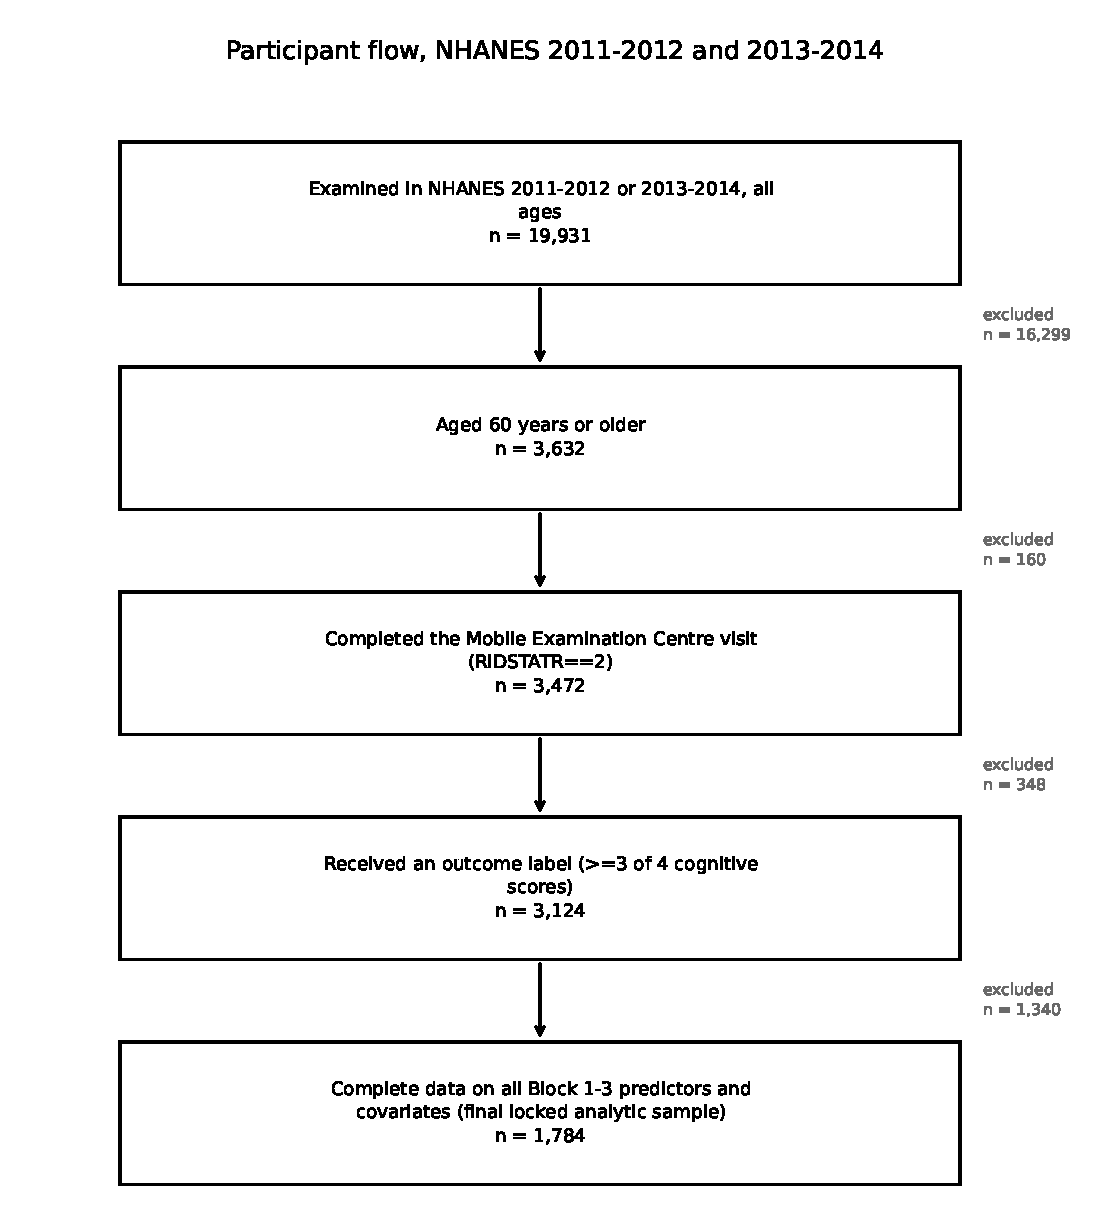
\includegraphics[width=0.85\textwidth]{figures/fig6_participant_flow.pdf}
\caption{Participant flow from NHANES 2011--2012 and 2013--2014 examined participants to the final locked analytic sample. Reasons for exclusion are given at each stage; the final step's exclusions (missing predictor data) are not mutually exclusive across blocks.}
\label{fig:flow}
\end{figure}

\begin{figure}[htbp]
\centering

\includegraphics[width=0.95\textwidth]{figures/fig1_delta_auc_forest.pdf}
\caption{Forest plot of \deltaauc\ contrasts with bootstrap 95\% confidence intervals: the four primary nested contrasts (M1$-$M0, M2$-$M0, M3$-$M0, M3$-$M0+) and the six pre-specified sensitivity analyses for M3$-$M0. Red markers indicate intervals excluding zero. The shaded band marks the pre-specified 0.02 meaningful-difference threshold.}
\label{fig:forest}
\end{figure}

\begin{figure}[htbp]
\centering

\includegraphics[width=0.7\textwidth]{figures/fig2_calibration.pdf}
\caption{Calibration, out-of-fold, by decile of predicted probability, for M0 (demographics), M3 (all biomarkers) and M0+ (clinical baseline). Calibration slope for each model is given in the legend; the dashed line is perfect calibration.}
\label{fig:calibration}
\end{figure}

\begin{figure}[htbp]
\centering
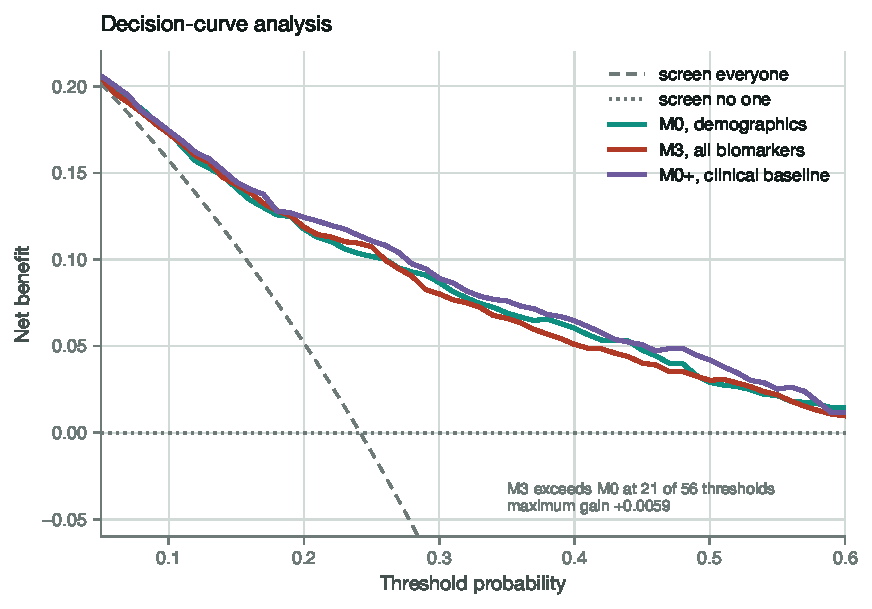
\includegraphics[width=0.85\textwidth]{figures/fig3_decision_curve.pdf}
\caption{Decision-curve analysis: net benefit against threshold probability for M0, M3 and M0+, against the treat-all and treat-none reference strategies.}
\label{fig:dca}
\end{figure}

\begin{figure}[htbp]
\centering

\includegraphics[width=0.9\textwidth]{figures/fig4_shap_rank_stability.pdf}
\caption{SHAP feature-importance rank stability across 200 bootstrap resamples of the gradient-boosted M3 model. Points are median rank, bars are the 95\% interval; the right-hand column gives the percentage of resamples in which each feature appeared in the top 5. Demographic predictors (purple) are essentially deterministic in rank; biomarkers (teal) are not.}
\label{fig:shap}
\end{figure}

\begin{figure}[htbp]
\centering
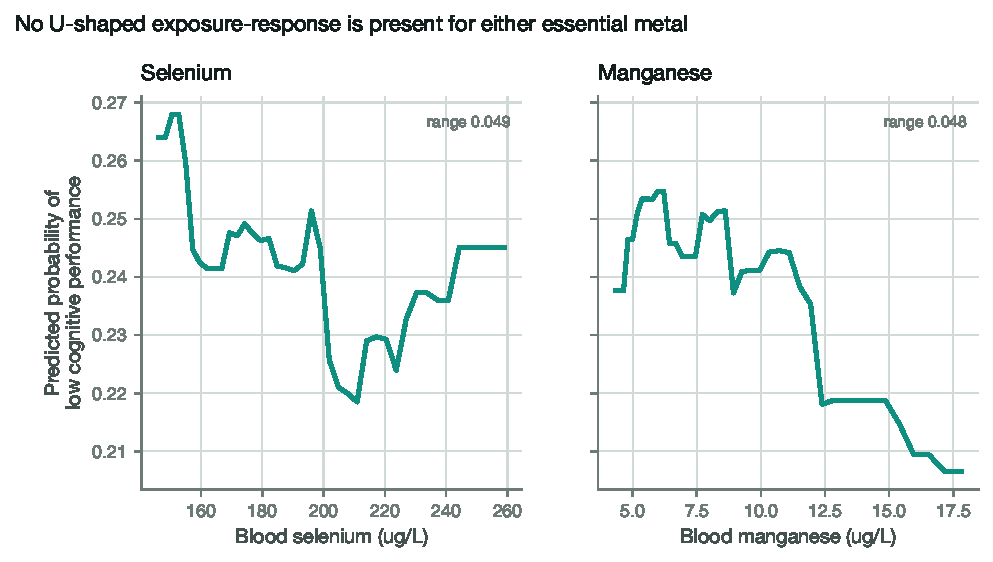
\includegraphics[width=0.9\textwidth]{figures/fig5_partial_dependence.pdf}
\caption{Partial dependence of predicted probability of low cognitive performance on blood selenium and blood manganese concentration (gradient-boosted M3 model), the two exposures for which a non-monotonic (U-shaped) exposure-response was anticipated in advance. Neither shows one; the predicted probability varies by approximately 0.05 across each exposure's observed range.}
\label{fig:pdp}
\end{figure}

\clearpage

% ============================================================
% TABLE 1
% ============================================================
\nolinenumbers
\begin{singlespace}
\footnotesize

\begin{longtable}{p{6.6cm}R{2.6cm}R{2.6cm}R{2.6cm}}
\caption{Participant characteristics, analytic sample ($n=1{,}784$), overall and by outcome status.}
\label{tab:t1a}\\
\toprule
Characteristic & Overall & Low cognitive performance & Not low cognitive performance \\
\midrule
\endfirsthead
\multicolumn{4}{l}{\textit{Table \ref{tab:t1a} continued}}\\
\toprule
Characteristic & Overall & Low cognitive performance & Not low cognitive performance \\
\midrule
\endhead
\bottomrule
\endfoot
\bottomrule
\endlastfoot
$n$ & 1784 & 431 & 1353 \\
Age, years, mean (SD) & 69.37 (6.74) & 72.07 (6.94) & 68.52 (6.44) \\
Income-to-poverty ratio, mean (SD) & 2.60 (1.60) & 1.91 (1.38) & 2.82 (1.61) \\
Blood lead, $\mu$g/dL, median [IQR] & 1.47 [1.01, 2.19] & 1.57 [1.03, 2.41] & 1.44 [1.01, 2.12] \\
Blood cadmium, $\mu$g/L, median [IQR] & 0.38 [0.25, 0.61] & 0.42 [0.27, 0.69] & 0.37 [0.25, 0.58] \\
Blood total mercury, $\mu$g/L, median [IQR] & 0.93 [0.49, 1.94] & 0.75 [0.40, 1.56] & 0.99 [0.53, 2.01] \\
Blood selenium, $\mu$g/L, median [IQR] & 193.09 [177.40, 208.38] & 188.35 [173.17, 204.15] & 194.23 [179.15, 209.06] \\
Blood manganese, $\mu$g/L, median [IQR] & 8.71 [6.90, 11.09] & 8.35 [6.50, 10.69] & 8.80 [7.02, 11.19] \\
Serum vitamin B12, pmol/L, median [IQR] & 410.30 [289.30, 601.45] & 421.40 [284.50, 621.80] & 408.10 [290.00, 599.30] \\
Serum methylmalonic acid, $\mu$mol/L, median [IQR] & 163.00 [125.75, 227.00] & 181.00 [131.00, 256.00] & 160.00 [124.00, 214.00] \\
Serum total folate, nmol/L, median [IQR] & 20.80 [13.60, 31.42] & 20.00 [13.05, 32.05] & 20.90 [13.70, 31.30] \\
RBC folate, nmol/L, median [IQR] & 543.00 [398.00, 737.00] & 530.00 [391.00, 748.50] & 547.00 [401.00, 733.00] \\
25-hydroxyvitamin D, nmol/L, mean (SD) & 76.31 (30.44) & 72.68 (30.36) & 77.46 (30.39) \\
HbA1c, \%, median [IQR] & 5.80 [5.50, 6.30] & 5.90 [5.50, 6.50] & 5.80 [5.50, 6.20] \\
HDL cholesterol, mg/dL, median [IQR] & 52.00 [43.00, 63.00] & 49.00 [40.00, 60.00] & 52.00 [44.00, 63.00] \\
Total cholesterol, mg/dL, mean (SD) & 192.85 (43.15) & 185.58 (41.41) & 195.16 (43.45) \\
Triglycerides, mg/dL, median [IQR] & 126.00 [86.00, 187.25] & 128.00 [91.00, 182.00] & 126.00 [85.00, 189.00] \\
Serum albumin, g/dL, mean (SD) & 4.20 (0.31) & 4.15 (0.34) & 4.21 (0.29) \\
Serum iron, $\mu$g/dL, median [IQR] & 80.00 [61.00, 103.00] & 76.00 [57.00, 96.00] & 82.00 [63.00, 104.00] \\
eGFR, mL/min/1.73\,m\textsuperscript{2}, mean (SD) & 75.64 (19.85) & 69.95 (22.19) & 77.45 (18.69) \\
Neutrophil-to-lymphocyte ratio, median [IQR] & 2.11 [1.55, 2.92] & 2.35 [1.67, 3.21] & 2.05 [1.53, 2.83] \\
Platelet-to-lymphocyte ratio, median [IQR] & 119.80 [94.11, 152.96] & 119.05 [89.76, 153.87] & 120.00 [95.26, 152.50] \\
Systemic immune-inflammation index, median [IQR] & 458.83 [319.14, 664.17] & 480.65 [322.90, 714.20] & 452.00 [315.00, 646.00] \\
Body mass index, kg/m\textsuperscript{2}, median [IQR] & 28.10 [24.77, 32.40] & 27.60 [24.30, 31.90] & 28.20 [24.90, 32.50] \\
Alcoholic drinks per day, median [IQR] & 0.00 [0.00, 1.25] & 0.00 [0.00, 1.00] & 1.00 [0.00, 2.00] \\
PHQ-9 depression score, median [IQR] & 1.00 [0.00, 4.00] & 2.00 [0.00, 6.50] & 1.00 [0.00, 4.00] \\
Sex = Male & 880 (49.3\%) & 238 (55.2\%) & 642 (47.5\%) \\
Sex = Female & 904 (50.7\%) & 193 (44.8\%) & 711 (52.5\%) \\
Race/ethnicity = Mexican American & 140 (7.8\%) & 46 (10.7\%) & 94 (6.9\%) \\
Race/ethnicity = Other Hispanic & 182 (10.2\%) & 68 (15.8\%) & 114 (8.4\%) \\
Race/ethnicity = Non-Hispanic White & 863 (48.4\%) & 165 (38.3\%) & 698 (51.6\%) \\
Race/ethnicity = Non-Hispanic Black & 425 (23.8\%) & 120 (27.8\%) & 305 (22.5\%) \\
Race/ethnicity = Non-Hispanic Asian & 144 (8.1\%) & 26 (6.0\%) & 118 (8.7\%) \\
Race/ethnicity = Other/multiracial & 30 (1.7\%) & 6 (1.4\%) & 24 (1.8\%) \\
Education = Less than 9th grade & 224 (12.6\%) & 137 (31.8\%) & 87 (6.4\%) \\
Education = 9--11th grade & 219 (12.3\%) & 79 (18.3\%) & 140 (10.3\%) \\
Education = High school grad/GED & 417 (23.4\%) & 103 (23.9\%) & 314 (23.2\%) \\
Education = Some college/AA degree & 511 (28.6\%) & 71 (16.5\%) & 440 (32.5\%) \\
Education = College graduate or above & 413 (23.2\%) & 41 (9.5\%) & 372 (27.5\%) \\
Smoking status = Never & 895 (50.2\%) & 210 (48.7\%) & 685 (50.6\%) \\
Smoking status = Former & 671 (37.6\%) & 159 (36.9\%) & 512 (37.8\%) \\
Smoking status = Current & 218 (12.2\%) & 62 (14.4\%) & 156 (11.5\%) \\
Ever told had a stroke & 125 (7.0\%) & 49 (11.4\%) & 76 (5.6\%) \\
Ever told had diabetes & 490 (27.5\%) & 154 (35.7\%) & 336 (24.8\%) \\
Ever told had high blood pressure & 1111 (62.3\%) & 302 (70.1\%) & 809 (59.8\%) \\
Ever told had high cholesterol & 997 (55.9\%) & 234 (54.3\%) & 763 (56.4\%) \\
\end{longtable}

\bigskip

\begin{longtable}{p{6.0cm}R{3.5cm}R{3.5cm}}
\caption{Included versus excluded participants, among the 3,124 outcome-eligible participants.}
\label{tab:t1b}\\
\toprule
Characteristic & Included ($n=1{,}784$) & Excluded ($n=1{,}340$) \\
\midrule
\endfirsthead
\toprule
Characteristic & Included ($n=1{,}784$) & Excluded ($n=1{,}340$) \\
\midrule
\endhead
\bottomrule
\endlastfoot
Age, years, mean (SD) & 69.37 (6.74) & 70.10 (6.94) \\
Income-to-poverty ratio, mean (SD) & 2.60 (1.60) & 2.50 (1.59) \\
PHQ-9 depression score, median [IQR] & 1.00 [0.00, 4.00] & 2.00 [0.00, 5.00] \\
Female, \% & 50.7\% & 52.6\% \\
Low cognitive performance, \% & 24.2\% & 26.1\% \\
Diabetes, \% & 27.5\% & 30.0\% \\
\end{longtable}

\end{singlespace}
\linenumbers

\clearpage

\doublespacing

% ============================================================
% DECLARATIONS
% ============================================================
\section*{Declarations}

\subsection*{Ethics approval and consent to participate}

NHANES protocol and procedures were approved by the National Center for Health Statistics (NCHS) Ethics Review Board (formerly the NCHS Research Ethics Review Board), and written informed consent was obtained from all participants by NCHS prior to data collection. This study is a secondary analysis of de-identified, publicly available data and involved no additional contact with participants. Both authors confirmed that their institutions (Davidson College and the University of North Carolina at Chapel Hill) impose no additional IRB requirement for this secondary analysis.

\subsection*{Consent for publication}

Not applicable. No individual person's data, images, or identifiable information are presented; all results are reported at the level of aggregate statistics on a de-identified public dataset.

\subsection*{Availability of data and materials}

NHANES data are publicly available from the CDC at wwwn.cdc.gov and are not redistributed here; the download script rebuilds the raw dataset from the original CDC URLs. The analysis code is available at \url{https://github.com/NeilP211/nhanes-ieee}, under version control, with every random seed fixed and every package version pinned.

\subsection*{Competing interests}

The authors declare that they have no competing interests.

\subsection*{Funding}

This research received no specific grant from any funding agency in the public, commercial, or not-for-profit sectors.

\subsection*{Authors' contributions}

S.K.\ and N.P.\ conceived the study and jointly decided the analytic sample definition, the nested model specification, and the pre-registration. S.K.\ acquired the raw data. N.P.\ curated the data and developed and ran the primary modelling pipeline: cohort construction, outcome construction, the nested M0--M3/M0+ models across three algorithms, cross-validated evaluation, interpretation (SHAP, partial dependence), and the six sensitivity analyses. S.K.\ conducted the literature review and citation verification, and conducted the participant flow-diagram, Table~\ref{tab:t1a}, and full model coefficient analyses. N.P.\ wrote the original draft of the Methods and Results; S.K.\ wrote the original draft of the Abstract, Introduction, and Discussion. Both authors reviewed and edited the complete manuscript and approved the final version. S.K.\ and N.P.\ contributed equally to this work and share first authorship.

\subsection*{Acknowledgements}

Not applicable.

% ============================================================
% REFERENCES
% ============================================================
\clearpage
\begin{singlespace}
\section*{References}

\begin{enumerate}
\item Wang N, Guo L, Shi M, Wang L, Zhou Y, Liu H, et al. Association of single and combined effects of blood heavy metals with cognitive function in older adults of the United States: a cross-sectional study. Research Square [Preprint]. 2024. Not confirmed as peer-reviewed at time of writing---cite as a preprint. Available from: \url{https://www.researchsquare.com/article/rs-4786268/v1}

\item Lu K, Liu T, Wu X, Zhong J, Ou Z, Wu W. Association between serum iron, blood lead, cadmium, mercury, selenium, manganese and low cognitive performance in old adults from National Health and Nutrition Examination Survey (NHANES): a cross-sectional study. Br J Nutr. 2023;130(10):1743--1753. \url{https://doi.org/10.1017/S0007114523000740}

\item Tang C, Shen M, Hong H. Uncovering the relationship between trace element exposure, cognitive function, and dietary inflammation index in elderly Americans from the National Health and Nutrition Examination Survey 2011--2014. BMC Public Health. 2024;24:2516. \url{https://doi.org/10.1186/s12889-024-20060-4}

\item Fu Z, Xu X, Cao L, Xiang Q, Gao Q, Duan H, et al. Single and joint exposure of Pb, Cd, Hg, Se, Cu, and Zn were associated with cognitive function of older adults. Sci Rep. 2024;14:28567. \url{https://doi.org/10.1038/s41598-024-79720-5}

\item Song S, Liu N, Wang G, Wang Y, Zhang X, Zhao X, et al. Sex specificity in the mixed effects of blood heavy metals and cognitive function on elderly: evidence from NHANES. Nutrients. 2023;15(13):2874. \url{https://doi.org/10.3390/nu15132874}

\item Laouali N, Benmarhnia T, Lanphear BP, Weuve J, Mascari M, Boutron-Ruault MC, et al. Association between blood metals mixtures concentrations and cognitive performance, and effect modification by diet in older US adults. Environ Epidemiol. 2022;6(1):e192. \url{https://doi.org/10.1097/EE9.0000000000000192}

\item Huang G, Ren G. Interaction between omega-6 fatty acids intake and blood cadmium on the risk of low cognitive performance in older adults from National Health and Nutrition Examination Survey (NHANES) 2011--2014. BMC Geriatr. 2022. \url{https://doi.org/10.1186/s12877-022-02988-7}

\item Ren F, Zhao X, Yang Q, Liao H, Zhang Y, Liu X. A machine learning framework for predicting cognitive impairment in aging populations using urinary metal and demographic data. Front Genet. 2025;16:1631228. \url{https://doi.org/10.3389/fgene.2025.1631228}

\item Nabavi A, Safari F, Kashkooli M, Nabavizadeh SS, Molavi Vardanjani H. Early prediction of cognitive impairment in adults aged 20 years and older using machine learning and biomarkers of heavy metal exposure. Curr Res Toxicol. 2024;7:100198. \url{https://doi.org/10.1016/j.crtox.2024.100198}

\item Collins GS, Moons KGM, Dhiman P, Riley RD, Beam AL, Van Calster B, et al. TRIPOD+AI statement: updated guidance for reporting clinical prediction models that use regression or machine learning methods. BMJ. 2024;385:e078378. \url{https://doi.org/10.1136/bmj-2023-078378}

\end{enumerate}
\end{singlespace}

\end{document}
